\documentclass[conference]{IEEEtran}
\IEEEoverridecommandlockouts
% The preceding line is only needed to identify funding in the first footnote. If that is unneeded, please comment it out.
\usepackage[numbers]{natbib}
\usepackage{amsmath,amssymb,amsfonts}
\usepackage{algorithmic}
\usepackage{graphicx}
\usepackage{textcomp}
\usepackage{xcolor}
\def\BibTeX{{\rm B\kern-.05em{\sc i\kern-.025em b}\kern-.08em
    T\kern-.1667em\lower.7ex\hbox{E}\kern-.125emX}}

\begin{document}
\title{Optimal stable coin folding strategy}

\author{\IEEEauthorblockN{Stefan Duprey, Frederic Fayes, Tom Suter, Matteo Bonatto}
\IEEEauthorblockA{\textit{SwissBorg} \\
stefan@swissborg.com, frederic@swissborg.com, tom@swissborg.com}
}

\maketitle

\begin{abstract}
A basic 'Lend/Borrow' strategy on the Aave protocol is one of the best and safest way to generate yield on your stable coins.\\
Those strategies are perfect fits for multiple 'Lend/Borrow' iterations or 'Folding' due to the inherent pegging of stable coins and the low liquidation risk incurred.\\
The question of the optimal $AUM$ allocation between multiple pools is a complex one.\\
APY dilution generate non linear effects, which can be solved through advanced non linear optimization algorithms/solvers, but those solvers are computationally intensive and won't transport easily into solidity code and limited computations due to high gas prices.\\
We here propose a linearization which give a simpler constrained quadratic optimization problem, whose solution can be expressed analytically through Lagrange multiplier.\\
That analytical solution can be seamlessly computed in solildity and live on a blockchain even with high gas prices.\\
\end{abstract}
\section{Folding strategy}

\begin{center}
\begin{tabular}{||c c c||} 
 \hline
 Iteration & Supply & Borrow \\ [0.5ex] 
 \hline\hline
 0 &  A & A*X  \\ 
 \hline
 1 &  A*X & A*X*X\\
 \hline
 ... & &  \\
 \hline
 n &  A*X^{n} & A*X^{n+1} \\
 \end{tabular}
\end{center}
The total amount supplied after $n$ iterations is:
\begin{equation}\label{eq:foldingSupply}
S = \sum\limits_{i=0}^{n} A*X^i = A\frac{1-X^{n+1}}{1-X} 
\end{equation}
$$
S \approx \sum\limits_{i=0}^{+\infty} A*X^n = A\frac{1}{1-X}
$$
The total amount borrowed after $n$ iterations is:
\begin{equation}\label{eq:foldingBorrow}
B = \sum\limits_{i=0}^{n} A*X^{i+1} = A*X\frac{1-X^{n+1}}{1-X}
\end{equation}
$$
B \approx \sum\limits_{i=0}^{+\infty} A*X^{n+1} = A\frac{X}{1-X}
$$
By defining the total APY on the supply side as the sum of the base APY and the liquidity incentive APY, here comes :
\begin{equation} \label{eq:tAPYsupply}
   \text{sAPY} = \text{supply APY} + \text{incentive supply APY} 
\end{equation}

\begin{equation}\label{eq:tAPYborrow}
  \text{bAPY} = \text{borrow APY} - \text{incentive borrow APY} 
\end{equation}

\begin{equation}
   \text{total APY} = \frac{A}{1-X} * sAPY - \frac{A*X}{1-X} * bAPY 
\end{equation}

This total APY is obviously strictly increasing as a function of the percentage ratio X.
\begin{equation}
\frac{d} {dX}\left( \text{total APY}\right) = \frac{\left(sAPY-bAPY\right)} {(1-X)^2}>0
\end{equation}
 The upper bound for X is only set by type of pools according to the incurred liquidation threshold.\\
 For stable coin pools with historicaly prooved pegging, $X$ can be chosen as high as $72\%$.

\section{Allocating between pools : an optimization problem}
\subsection{Aave protocol : a trade off to maximize utilization/assured withdrawal }
Aave protocol implements at its core a regulating mechanism which aims at maximizing profits for liquidity supplier while keeping them safe and always able to withdraw their liquidity.\\
The utilization rate, which is just the ratio of the total borrowed divided by the total supplied:
\begin{equation}
U = \frac{B_t}{L_t}
\end{equation}
is algorithmically targeted to stay close to an optimal $U_{optimal}$ fixed by Aave governance per different pools. \\
The targeting mechanism can be summed up to the definition of two different borrow rate growth regime according to the value of U under or above U_{optimal}.\\\\
$$
R_b=\left\{
\begin{array}{ll}
  R_{b_0} + \frac{U}{U_{optimal}} * R_{slope1}\text{, if } U \le U_{optimal}\\
  R_{b_0}+ R_{slope1} + \frac{U-U_{optimal}}{1-U_{optimal}} * R_{slope2}, \text{ } U\ge U_{optimal} 
\end{array}
\right.
$$\\\\\\
$R_b$ is the borrow rate, which will rise sharply after $U>U_{optimal}$ to prevent the ratio from being too close to one, which could keep suppliers from withdrawing their fund.\\
$R_{b0}$ is the constant base variable borrow rate.\\
The supply rate is then defined as the borrow rate multiplied by the utilization ratio.
\begin{equation}
R_s = R_b * U
\end{equation}
The greater the utilization ratio, the more yield suppliers will get. 
\begin{equation}
R_s - R_b = R_b * (U-1) <0
\end{equation}

\subsection{Stable coin pool parameters}
Aave protocol governance has assigned the following parameters all common across stable pool reserves :
\begin{center}
\begin{tabular}{||c c c c c||} 
 \hline
 Coin & U_{optimal} & base & slope1 & slope2 \\ [0.5ex] 
 \hline\hline
 DAI & 90\% & 0\% & 4\% & 60\% \\ 
 \hline
 USDC &  90\% & 0\% & 4\% & 60\% \\
 \hline
 USDT &  90\% & 0\% & 4\% & 60\%\\
 \end{tabular}
\end{center}

\subsection{Liquidity incentives APR}
\subsubsection{Definition}
The definition of the liquidity incentives can be found in Aave V2 protocol white paper :

\begin{equation}\label{eq:isAPR}
 isAPR=100 *\frac{ aEmissionPerYear* rewardPrice}{totalATokenSupply * tokenPrice} 
\end{equation}
where the parameters match the following in the smart contract are detailed in the solidity section\\

\begin{equation}\label{eq:ibAPR}
 ibAPR=100 *\frac{ vEmissionPerYear* rewardPrice}{totalCurrentVariableDebt * tokenPrice} 
\end{equation}
where the parameters match the following in the smart contract are detailed in the solidity section\\

We see that from the assumption of a fixed reward price and emission rate, the borrow APR depends on the total current debt :\\
\begin{equation}
APR_b = \frac{cte_b}{B_t}
\end{equation}\\
And the supply APR depends on the total liquidity:\\
\begin{equation}
APR_s = \frac{cte_s}{L_t}
\end{equation}
\subsubsection{Compounding}
We will here assume that those incentive annual $APR$ are indeed harvested and reinvested in the strategy leading to an annualized compounded APY:
\begin{equation}\label{eq:APRtoAPY}
APY = (1+ \frac{APR}{secondsPerYear})^{secondsPerYear}-1
\end{equation}
The reverse equation is :
\begin{equation}
APR = ((1+ APY)^{\frac{1}{secondsPerYear}}-1)*secondsPerYear
\end{equation}


\subsection{Dilution effect}
When a proportion $X$ of an additional amount $AUM$ is dispatched to a specific liquidity pool. This pool will incur a dilution effect on its liquidity.\\
$L_t \leftarrow L_t + X*AUM$\\


\subsection{First order approximation}
We can simplify the non linear term under the assumption: \\
$$
\frac{1}{L_t + X*AUM} = \frac{1}{L_t } *\frac{1}{1 + \frac{X}{\frac{L
_t}{AUM}}} = \frac{1}{L_t } * \sum_{n=0}^{n=+\infty}(-1)^n\frac{X^n}{\frac{L
_t}{AUM}^{n}}
$$
If $X<<\frac{L_t}{AUM}$, as a first order approximation:
$$
\frac{1}{L_t + X*AUM}  = \frac{1}{L_t }  - \frac{AUM}{L_t^2} * X 
$$
Here comes the new diluted utilization ratio :\\ 
\begin{equation}\label{eq:diluted_ratio}
U(X) = \frac{B_t}{L_t + X*AUM} = \frac{B_t}{L_t } *\frac{1}{1 + \frac{X}{\frac{L
_t}{AUM}}} \approx \frac{B_t}{L_t }*( 1 -\frac{X}{\frac{L
_t}{AUM}})
\end{equation}
Here comes the new diluted incentive APYs:\\ 
\begin{equation}\label{eq:diluted_APR}
APR_s(X) = \frac{cte_s}{L_t + X*AUM}  \approx  cte_s * ( \frac{1}{L_t }  - \frac{AUM}{L_t^2} * X )
\end{equation}
After multiple folding \label{eq:foldingSupply} and \label{eq:foldingBorrow}, we then linearize as in \ref{eq:diluted_APR}\\
It comes after linearization :\\
$$
APR(X) = APR_s(X) + APR_s(X)\\ 
$$
$$
= \frac{cte_s}{L_t + \frac{X*AUM}{1-X_{leverage}}}+ \frac{cte_b}{B_t + \frac{X_{leverage}*X*AUM}{1-X_{leverage}}}  \\
$$
$$
\approx  cte_s * ( \frac{1}{L_t}  - \frac{AUM}{L_t^2} * X )
$$
\begin{equation}\label{eq:linear_APR}
APR(X) \approx A_0 + A_1*X
\end{equation}
where 
\begin{equation}\label{eq:A_0}
A_0 = \frac{cte_s}{L_t} + \frac{cte_b}{B_t}
\end{equation}
\begin{equation}\label{eq:A_1}
A_1 = -\frac{cte_s*AUM}{L_t^2*(1-X_{leverage})} -\frac{cte_b*AUM*X_{leverage}}{B_t^2*(1-X_{leverage})}
\end{equation}

\subsection{Optimization problem}
When having to allocate an amount $AUM$ between $n$ pools, one will look at optimizing the total generated yield :  
\begin{equation}
 \left( \omega_1,...,\omega_n \right)   =  \arg \max_{ \sum_{i = 1}^{i = n} \omega_i = 1,0\le \omega_i \le 1} { \sum_{i = 1}^{i = n} \omega_i \times tAPY_i\left(\omega_i * AUM \right) }
\end{equation}
where the total APYs $APY_i$ for each pool i are defined in equations \ref{eq:tAPYsupply} and \ref{eq:tAPYborrow}.\\
The \ref{eq:APRtoAPY} equation shows that the liquidity incentive APYs on Aave are actually the main prominent reason for choosing a specific pool.\\
We can in a first approximation try to solve the simpler problem :
\begin{equation}\label{eq:optim}
 \left( \omega_1,...,\omega_n \right)   =  \arg \max_{ \sum_{i = 1}^{i = n} \omega_i = 1,0\le \omega_i \le 1} { \sum_{i = 1}^{n} \omega_i \times APR_i\left(\omega_i * AUM \right) }
\end{equation}
\subsection{Constrained quadratic optimization for the linearized problem}
Under the conditions $X<<\frac{L_t}{AUM}$ and $U<U_{optimal}$, by using the first order approximations \ref{eq:linear_APR} :
$$
 \left( \omega_1,...,\omega_n \right)   =  \arg \max_{ \sum_{i = 1}^{i = n} \omega_i = 1,0\le \omega_i \le 1} { \sum_{i = 1}^{n} \omega_i \times \left( {A_0}_i   + {A_1}_i * \omega_i\right) }
$$
where ${A_0}_i$, ${A_1}_i$ are the constants for the pool $i$.\\
By calling
$$
J(x)=- \sum_{i = 1}^{n} x_i \times \left( {A_0}_i   + {A_1}_i * x_i \right)
$$
The optimization problem becomes a constrained quadratic minimization problem
$$
\min\limits_{\sum x_i =1,0\le x_i \le 1} {J(x)}
$$
\subsection{Analytical solution from Lagrange multiplier}
By rewriting the constraint as :
$$
g(x) = \sum_{i = 1}^{n} x_i
$$
We can compute the optimal solution using the Lagrange multiplier and the modified functional taking into the equality constraints and the inequality constraints using KKT conditions and slack variables:

$$
J'(x)=J(x) + \lambda \left( g(x) - 1\right)
$$
$$
+\sum_i \theta_i*(x_i- s_i^2)+\sum_i \gamma_i*(1-t_i^2-x_i)
$$
We solve the Lagrangian equations :
\begin{equation}
\left\{
\begin{array}{ll}
  \nabla_x J'(x) = 0\\
  \nabla_\lambda J'(x)= 0 \\
  \nabla_\theta J'(x)= 0 \\
\end{array}
\right.
\end{equation}
The $\nabla_x$ conditions give the following :
$$
\begin{pmatrix} 
	{A_0}_1 + 2*{A_1}_1 * x_1  + \lambda + \theta_1 -\gamma_1\\
	\vdots\\
	{A_0}_i + 2*{A_1}_i * x_i  + \lambda + \theta_i-\gamma_i\\
	\vdots\\
	{A_0}_n + 2*{A_1}_n * x_n  + \lambda + \theta_n-\gamma_n\\
\end{pmatrix} 
=
\begin{pmatrix} 
	0 \\
	\vdots\\
	0 \\
	\vdots\\
	0 \\
	\end{pmatrix} 
$$
First case, if all $\theta_i$ and $\gamma_i$ are null, it means that all slack variables $s_i^2$ and $t_i^2$ are positive and the constraints are not active.\\
The $x$ solution reads :
\begin{equation}\label{eq:constraintsnotbroken}
\forall i \in \left[1,\ldots,n\right], x_i = -\frac{\lambda + {A_0}_i}{2*{A_1}_i}
\end{equation}
and the Lagrange multiplier can then be quantified through the constraint :
\begin{equation}\label{eq:lambda}
\lambda =\frac{-1 -\sum_{i=1}^{n} \frac{{A_0}_i}{2*{A_1}_i}} {\sum_{i=1}^{n} \frac{1}{2*{A_1}_i}}
\end{equation}
In the case where on one $x_i$ does not respect the inequalities, it means that either 
$x_i = 1 or 0$ depending on if $\theta_i$ or $\gamma_i$ is not null.
The solution is then obtained recursively by reiterating the \ref{eq:constraintsnotbroken} and \ref{eq:lambda} with the remaining $x_i$s until all are found respecting the inequalities.
\section{Allocating between pools : an optimization problem}
We here present optimization results for the following snapshot parameter for a three pools (DAI, USDC, USDT) allocation on Aave Avalanche.
\begin{figure}[h!]
    \centering
    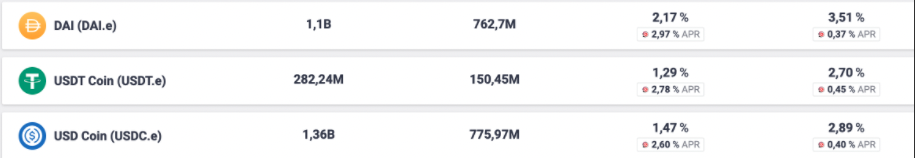
\includegraphics[scale=0.25]{Plots/optim_params.png}
    \caption{Optimization parameters}
    \label{fig:optim_params}
\end{figure}
\begin{figure}[h!]
    \centering
    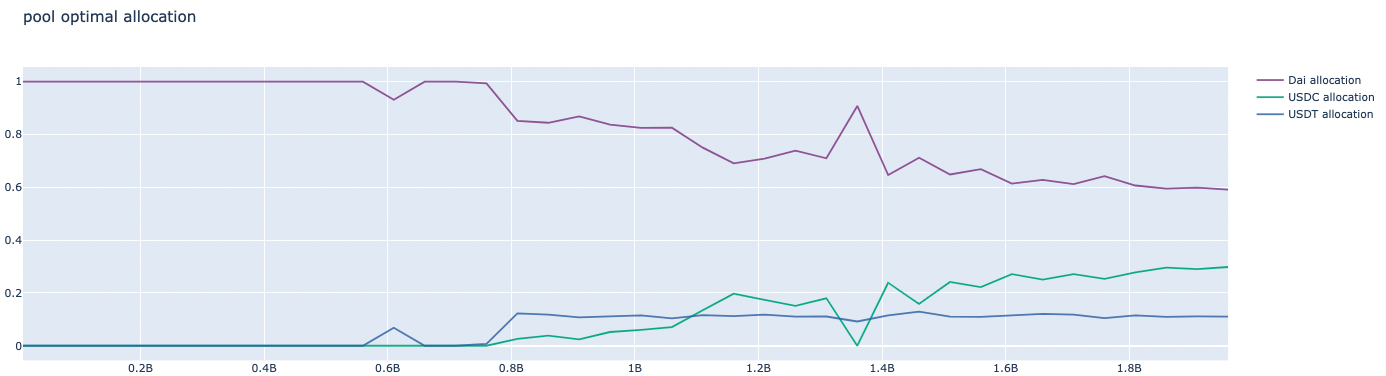
\includegraphics[scale=0.19]{Plots/nonlinear.png}
    \caption{Non linearized exact solution}
    \label{fig:nonlinear}
\end{figure}
\subsection{}
\begin{figure}[h!]
    \centering
    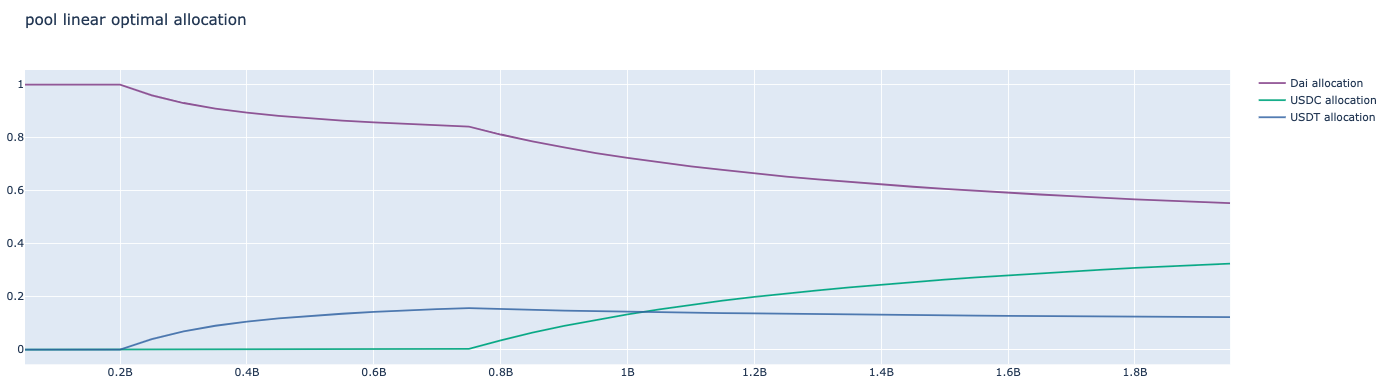
\includegraphics[scale=0.19]{Plots/linearized_quadratic.png}
    \caption{Approximative linearized solution}
    \label{fig:linearized_quadratic}
\end{figure}

\section{Solidity code for optimization}
The new diluted incentive APYs expression \ref{eq:diluted_APR} and both equations \ref{eq:ibAPR} and \ref{eq:isAPR} give us the expression for our ${A_0}_i$ and ${A_1}_i$

\begin{equation}
 isAPR=100 *\frac{a*r*w}{L_t*t*d} =\frac{cte_s}{L_t}
\end{equation}
where $cte_s = 100 *\frac{a*r*w}{t*d}$ the parameters match the followings in the smart contract :\\
$$
\left\{
\begin{array}{c}
  isAPR=incentiveDepositAPRPercent\\
  a=aEmissionPerYear\\
  r=REWARDPRICEETH \\
  w=WEIDECIMALS\\
  t=TOKENPRICEETH \\
  d=TOKENDECIMALS\\
  L_t =totalATokenSupply\\
\end{array}
\right.
$$

\begin{equation}\label{eq:ibAPR}
 ibAPR=100 *\frac{v *r*w}{B_t*t*d}=\frac{cte_b}{B_t} 
\end{equation}
where $cte_b = 100 *\frac{v *r*w}{t*d}$ the parameters match the followings in the smart contract :\\
$$
\left\{
\begin{array}{c}
  ibAPR=incentiveBorrowAPRPercent\\
  v=vEmissionPerYear\\
  r=REWARDPRICEETH \\
  w=WEIDECIMALS\\
  B_t=totalCurrentVariableDebt\\
  t=TOKENPRICEETH \\
  d=TOKENDECIMALS\\
\end{array}
\right.
$$\\

By using equations \ref{eq:A_1} and \ref{eq:A_0}, we can compute ${A_0}_i$ and ${A_1}_i$ for each pool. \\
Equations \ref{eq:lambda} and \ref{eq:x_i} give us then the optimal pool allocation.\\

\section{Multi-protocol optimal allocation}
\subsection{Global optimization}
We here make the assumption that each protocol yield is shared with each participant according to the pro rata of their liquidity participation.\\
The $APY$ of protocol $i$ at time $t$ can be computed as :\\
\begin{equation}
APY_{i}(t) = \frac{fees_i(t)}{L_i(t)}
\end{equation}
We forgot the t parameter as protocol yield and liquidity as those are fixed when we rebalance at a specific time $t$ . When distributing our liquidity $AUM$ over
$i \in \left(1,..,n\right)$, each protocol APY $i$ can be computed as :
\begin{equation}
APY_{i} = \frac{fees_i}{L_i + \omega_i * AUM}
\end{equation}
where $\left( \omega_1,...,\omega_n \right)$ are the liquidity proportions attributed to each protocol.\\
We rewrite \ref{eq:optim} as one more general of a multi-protocol allocation constrained optimization problem :
\begin{equation}\label{multiprotocolallocation}
 \left( \omega_1,...,\omega_n \right)   =  \arg \max_{ \sum_{i = 1}^{i = n} \omega_i = 1,0\le \omega_i \le 1} { \sum_{i = 1}^{n} \omega_i \times APR_i\left(\omega_i * AUM \right) }
\end{equation}
\subsection{Risk consideration}
The constraint on weights :
\begin{equation}
0\le \omega_i \le 1, \forall i \in \left(1,..,n\right)
\end{equation}
can be taylored by tighter bounds which result from a protocol risk assessing methodology :
\begin{equation}\label{gogogo}
l_i \le \omega_i \le u_i, \forall i \in \left(1,..,n\right)
\end{equation}
where $u_i$ is the maximal proportion of liquidity we can afford for this protocol after a careful risk assessment and $l_i$ a diversification bound which can be null or common for all protocols $i$.
\section{Conclusion}
We have managed to simplify the optimization problem and transport it to EVM like blockchain languages.\\
The solution can scale up to at least ten pools without being too computationally intensive.\\
\bibliographystyle{IEEEtranN}
\bibliography{bib}
\nocite{*}
\end{document}

% to do
% Expliquer l'importance de la réduction de dimension dans ML
% Expliquer la diff CCA PCA pour ML